\documentclass[notes]{beamer}
\usepackage{hyperref}
\usepackage{graphicx}
%%%%%%%%%%%%%%%%%%%%%%%%%%%%%%%%%%%%%%%%%%%%%%%%%%%%%%%%%%%%%%%%
%% ccBeamer 0.1, 2007-07-02                                   %%
%% Written by Sebastian Pipping <webmaster@hartwork.org>      %%
%% ---------------------------------------------------------- %%
%% Licensed under Creative Commons Attribution-ShareAlike 3.0 %%
%% http://creativecommons.org/licenses/by-sa/3.0/             %%
%%%%%%%%%%%%%%%%%%%%%%%%%%%%%%%%%%%%%%%%%%%%%%%%%%%%%%%%%%%%%%%%


%% Images
\newcommand{\CcImageBy}[1]{%
	
\includegraphics[scale=#1]{creative_commons/cc_by_30.pdf}%
}
\newcommand{\CcImageCc}[1]{%
	
\includegraphics[scale=#1]{creative_commons/cc_cc_30.pdf}%
}
\newcommand{\CcImageDevNations}[1]{%
	\includegraphics[scale=#1]{creative_commons/cc_dev_nations_30.pdf}%
}
\newcommand{\CcImageNc}[1]{%
	\includegraphics[scale=#1]{creative_commons/cc_nc_30.pdf}%
}
\newcommand{\CcImageNd}[1]{%
	\includegraphics[scale=#1]{creative_commons/cc_nd_30.pdf}%
}
\newcommand{\CcImagePd}[1]{%
	\includegraphics[scale=#1]{creative_commons/cc_pd_30.pdf}%
}
\newcommand{\CcImageSa}[1]{%
	
\includegraphics[scale=#1]{creative_commons/cc_sa_30.pdf}%
}
\newcommand{\CcImageSampling}[1]{%
	\includegraphics[scale=#1]{creative_commons/cc_sampling_30.pdf}%
}
\newcommand{\CcImageSamplingPlus}[1]{%
	\includegraphics[scale=#1]{creative_commons/cc_sampling_plus_30.pdf}%
}


%% Groups
\newcommand{\CcGroupBy}[1]{% zoom
	\CcImageBy{#1}%
}
\newcommand{\CcGroupByNc}[2]{% zoom, gap
	\CcImageBy{#1}\hspace*{#2}\CcImageNc{#1}%
}
\newcommand{\CcGroupByNcNd}[2]{% zoom, gap
	\CcImageBy{#1}\hspace*{#2}\CcImageNc{#1}\hspace*{#2}\CcImageNd{#1}%
}
\newcommand{\CcGroupByNcSa}[2]{% zoom, gap
	\CcImageBy{#1}\hspace*{#2}\CcImageNc{#1}\hspace*{#2}\CcImageSa{#1}%
}
\newcommand{\CcGroupByNd}[2]{% zoom, gap
	\CcImageBy{#1}\hspace*{#2}\CcImageNd{#1}%
}
\newcommand{\CcGroupBySa}[2]{% zoom, gap
	\CcImageBy{#1}\hspace*{#2}\CcImageSa{#1}%
}
\newcommand{\CcGroupDevNations}[1]{% zoom
	\CcImageDevNations{#1}%
}
\newcommand{\CcGroupNcSampling}[2]{% zoom, gap
	\CcImageNc{#1}\hspace*{#2}\CcImageSampling{#1}%
}
\newcommand{\CcGroupPd}[1]{% zoom
	\CcImagePd{#1}%
}
\newcommand{\CcGroupSampling}[1]{% zoom
	\CcImageSampling{#1}%
}
\newcommand{\CcGroupSamplingPlus}[1]{% zoom
	\CcImageSamplingPlus{#1}%
}


%% Text
\newcommand{\CcLongnameBy}{Attribution}
\newcommand{\CcLongnameByNc}{Attribution-NonCommercial}
\newcommand{\CcLongnameByNcNd}{Attribution-NoDerivs}
\newcommand{\CcLongnameByNcSa}{Attribution-NonCommercial-ShareAlike}
\newcommand{\CcLongnameByNd}{Attribution-NoDerivs}
\newcommand{\CcLongnameBySa}{Attribution-ShareAlike}

\newcommand{\CcNote}[1]{% longname
	This work is licensed under the \textit{Creative Commons #1 3.0 License}.%
}

\mode<article>
    {
      \usepackage{fullpage}
      \usepackage{pdf}
      \usepackage{hyperref}
    }
    
\mode<presentation>{
  \usetheme{Dresden}
  \setbeamercovered{transparent}
}

\title{HacDC}
\author{Serge Wroclawski}
\begin{document}
\section{Introduction}

\begin{frame}
        \titlepage
        \vfill
        \begin{center}
                
\includegraphics{hacdc-logo}
                \CcGroupBySa{0.83}{0.95ex}\\[2.5ex]
                {\tiny\CcNote{\CcLongnameBySa}}
                \vspace*{-2.5ex}
                
\includegraphics{hacdc-logo}
        \end{center}
\end{frame}

\section{The Objective}

\begin{frame}
  \frametitle{What is HacDC?}
  From \href{http://www.hacdc.org}{hacdc.org}:
  \begin{quote}
    HacDC is a non-profit organization and space dedicated to
    technical, artistic and social collaboration. We are
    technologists, tinkerers, crafters and codemonkeys who call DC
    home. We collaborate across disciplines for the benefit of
    cultural, charitable and scientific causes. We create, learn and
    teach as a group, inviting our neighbors around the block and
    around the world to join us.
  \end{quote}
\end{frame}

\begin{frame}
  \frametitle{Does HacDC Do?}
  \begin{itemize}
  \item Provides a workshop for people to work on ongoing projects
  \item New Workshop Coming Soon!
  \item Provides a meeting space for groups
  \item An organization to bring communities together
  \end{itemize}
\end{frame}

\begin{frame}
  \frametitle{Does HacDC Do?}
  \begin{itemize}
  \item Provides a workshop for people to work on ongoing projects
  \item New Workshop Coming Soon!
  \item Provides a meeting space for groups
  \item An organization to bring communities together
  \end{itemize}
\end{frame}

\section{The Space}

\begin{frame}[fragile]
  \frametitle{The Space!}
  \begin{center}
    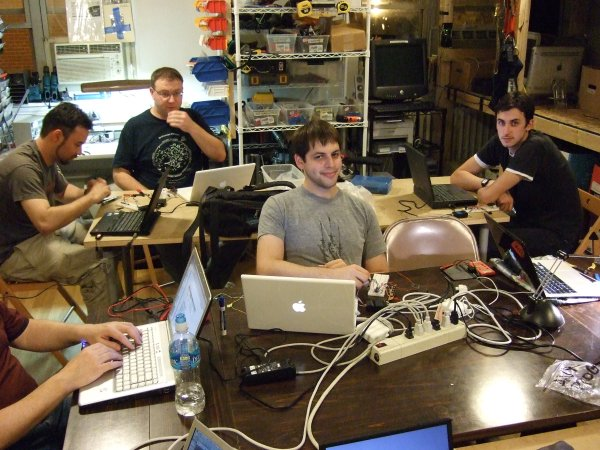
\includegraphics[width=.8\textwidth,height=.8\textheight]{dscf2730_small.jpg} \\
    {\em A classroom full of people on Microcontroller Mondays.}
  \end{center}
\end{frame}

\begin{frame}
  \frametitle{The Significance of the Space}
  \begin{itemize}
  \item The main differiantor between HacDC and other groups
  \item Teaching Space
  \item Workshop
  \item Social Space
  \item Open 24/7
  \end{itemize}
\end{frame}

\section{The Activities}

\begin{frame}
  \frametitle{HacDC Activities}
  \begin{itemize}
  \item Classes
  \item Weekly Talks
  \item Group Meetings/Project Gatherings
  \item Special Events
   \item Social Gatherings
   \end{itemize}
\end{frame}

\section{Future Plans}

\begin{frame}
  \frametitle{Future Plans}
  \begin{itemize}
  \item More Classes
  \item More Special Events
  \item More Community Service
  \end{itemize}
\end{frame}

\section{Getting Involved}

\begin{frame}
  \frametitle{Getting Involved}
  \begin{itemize}
  \item Go to \href{http://hacdc.org}{hacdc.org}
    \begin{itemize}
    \item Read the blog
    \item See/subscribe to the calendar
    \item Get on the announce or blabber lists
    \end{itemize}
  \item Go to our events
    \begin{itemize}
    \item They're all free and open to the public
    \end{itemize}
  \item Become a member
    \begin{itemize}
    \item Access to the workshop
    \item Hold meetings
    \item Help shape the organization
    \end{itemize}
  \end{itemize}
\end{frame}

\section{Questions}

\begin{frame}
  \begin{center}
    {\Large Questions?}
  \end{center}
\end{frame}

\section{Thanks and License}

\begin{frame}
  \vfill
  Special Thanks to:\\
  Tim Collins, Mitch Altman and Elliot Williams for the great photographs
  \\
  To DCLUG for providing me a forum for more than twelve years.
  And to HacDC for inspiration for this talk.
  \\
  Copyright \copyright 2009 Serge Wroclawski
  \\
  This presentation is available under the Creative Commons
  Attribution-ShareAlike License.
  \\
  Hac
  
  Current versions of this presentation are available at:
\end{frame}

\end{document}